\documentclass{article}
\usepackage{graphicx} % Required for inserting images
\usepackage[left=1.5cm, right=2cm, top=2cm, bottom=2cm]{geometry}
\usepackage[T1]{fontenc}    %  (ą, ł, ś)
\usepackage[utf8]{inputenc} %  UTF-8
\usepackage[colorlinks=true, linkcolor=black,citecolor=black]{hyperref}
\usepackage[polish]{babel}
\usepackage[polish]{cleveref}
\usepackage{array}
\usepackage{float}
\usepackage{makecell}
\usepackage{multirow}
\usepackage{amsmath}
\usepackage{gensymb}
\usepackage[table]{xcolor}
\documentclass[12pt]{article}
\setlength{\intextsep}{5pt}   
\setlength{\floatsep}{3pt}     
\setlength{\textfloatsep}{5pt} 
\crefname{figure}{Rys.}{Rys.}
\Crefname{figure}{Rys.}{Rys.}
\crefname{section}{Rozd.}{Rozdziały}
\Crefname{section}{Rozd.}{Rozdziały}


\title{
\includegraphics[width=0.5\textwidth]{obrazy/logo-pwr-wm.png}\\[0.2cm] \Huge Sprawozdanie z Fizyki \\[0.2cm] \Huge Ćwiczenie 20a}
\author{\Large t0f1x}

\date{Wrocław, xx.xx.202x, Grupa nr. x}
\begin{document}
\maketitle
\tableofcontents
\newpage
\section{Wstęp}
\label{Wstep}
Ćwiczenie ma na celu skalowanie termopary oraz wyznaczenie współczynnika termoelektrycznego
termopary. Skalowanie to proces wyznaczenia zależności napięcia termoelektrycznego, mierzonego w układzie termopary od zmienianej temperatury na jednym ze złącz, podczas gdy drugie złącze jest utrzymywane w stałej temperaturze ok. 0 $[^\circ\text{C}]$.  \\

Działanie termopary opiera się na zjawisku Seebecka, które polega na powstawaniu siły elektromotorycznej (napięcia termoelektrycznego) w obwodzie składającym się z dwóch różnych przewodników, gdy ich złącza znajdują się w różnych temperaturach. Zgodnie z teorią, badana zależność napięcia od temperatury powinna mieć charakter liniowy, co należy sprawdzić. \\
Podczas ćwiczenia stosowane są następujące przyrządy: Termopara, Multimetr Sanwa PC7000, kuchenka elektryczna, Termometr, naczynie do podgrzewania wody, termos z roztworem lodu i wody. \\


\newpage
\section{Wyniki}
\begin{table}[H]
    \centering
    \renewcommand{\arraystretch}{1.2}
    \resizebox{0.9\textwidth}{!}{
        \begin{tabular}{|c|c|c|c|c|c|c|c|c|}
        \hline
        \makecell{$T$ \\ $[^\circ\text{C}]$} & \makecell{$u(T)$ \\ $[^\circ\text{C}]$} & \makecell{$U$ \\ $[\text{mV}]$} & \makecell{$u(U)$ \\ $[\text{mV}]$} & \makecell{$\alpha$ \\ $[\text{mV}/^\circ\text{C}]$} & \makecell{$u(\alpha)$ \\ $[\text{mV}/^\circ\text{C}]$} & \makecell{$\frac{u(\alpha)}{\alpha} \cdot 100\%$ \\ $[\%]$} & \makecell{$B$ \\ $[\text{mV}]$} & \makecell{$u(B)$ \\ $[\text{mV}]$} \\ \hline
        33 & \multirow{15}{*}{0,058} & 1,30 & \multirow{15}{*}{0,0115} & \multirow{15}{*}{0,04239} & \multirow{15}{*}{0,00050} & \multirow{15}{*}{1,18\%} & \multirow{15}{*}{0,1204} & \multirow{15}{*}{0,0233} \\ \cline{1-1} \cline{3-3}
        35 &  & 1,38 &  &  &  &  &  &  \\ \cline{1-1} \cline{3-3}
        37 &  & 1,46 &  &  &  &  &  &  \\ \cline{1-1} \cline{3-3}
        39 &  & 1,53 &  &  &  &  &  &  \\ \cline{1-1} \cline{3-3}
        41 &  & 1,62 &  &  &  &  &  &  \\ \cline{1-1} \cline{3-3}
        43 &  & 1,70 &  &  &  &  &  &  \\ \cline{1-1} \cline{3-3}
        45 &  & 1,77 &  &  &  &  &  &  \\ \cline{1-1} \cline{3-3} 
        47 &  & 1,87 &  &  &  &  &  &  \\ \cline{1-1} \cline{3-3}
        49 &  & 1,95 &  &  &  &  &  &  \\ \cline{1-1} \cline{3-3}
        51 &  & 2,03 &  &  &  &  &  &  \\ \cline{1-1} \cline{3-3}
        53 &  & 2,15 &  &  &  &  &  &  \\ \cline{1-1} \cline{3-3}
        55 &  & 2,21 &  &  &  &  &  &  \\ \cline{1-1} \cline{3-3}
        57 &  & 2,27 &  &  &  &  &  &  \\ \cline{1-1} \cline{3-3}
        58 &  & 2,35 &  &  &  &  &  &  \\ \cline{1-1} \cline{3-3}
        60 &  & 2,44 &  &  &  &  &  &  \\ \cline{1-1} \cline{3-3}
        35,7 & & 1,35 & &  &  &  &  & \\ \cline{1-1} \cline{3-3}
        35 &  & 1,37 &  &  &  &  &  & \\ \hline
        \end{tabular}
    }
    \caption{Wyniki skalowania termopary}
    \label{tab:termopara}
\end{table}

\begin{figure}
    \centering
    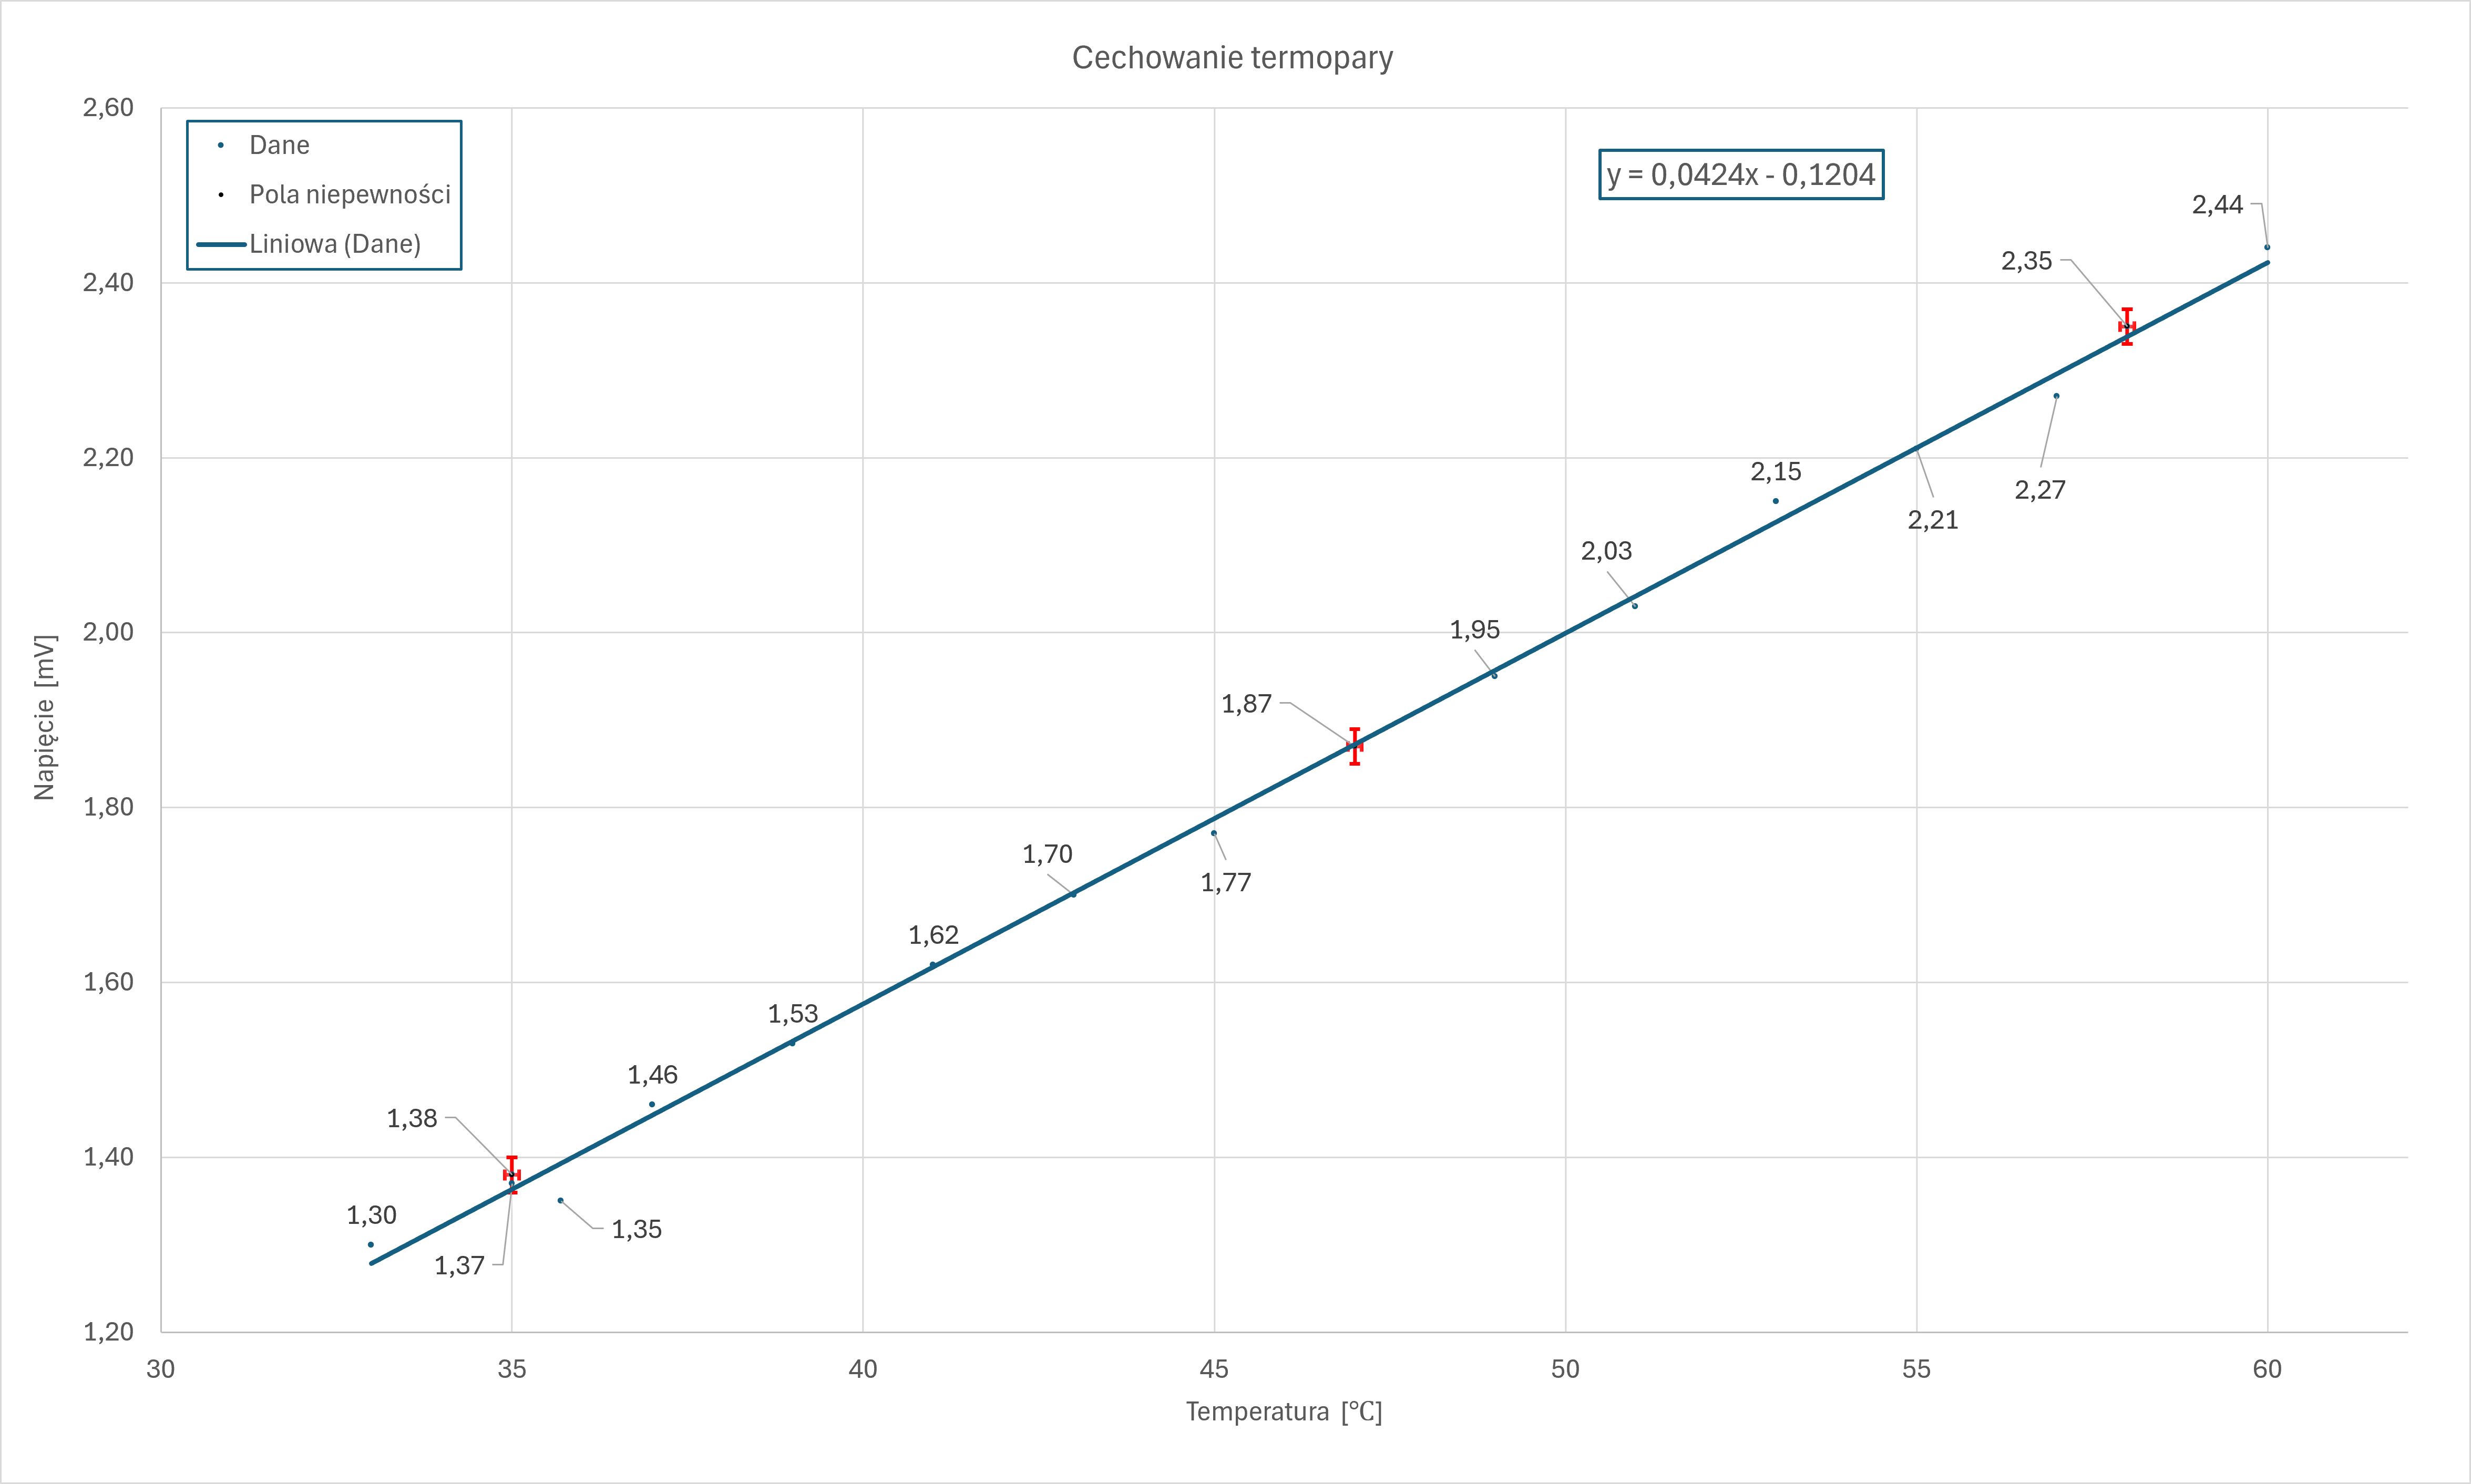
\includegraphics[angle=270, width=0.78\linewidth]{obrazy/Wykres.png}
    \caption{Wykres cechowania termopary}
    \label{fig:wykres}
\end{figure}

\newpage
\section{Obliczenia}
    \subsection{\centering Niepewności pomiarowe temperatury \ \(T\) }
        \subsubsection{Niepewność standardowa typu B}
                \begin{flalign*}
                    u_B(T)=\sqrt{\frac{\bigtriangleup_p^2(T)}{3}}=\frac{0,1}{\sqrt{3}}=0,058 \ [^\circ\text{C}] &&
                \end{flalign*}
    \subsection{\centering Niepewności pomiarowe napięcia \ \(U\) }
    \begin{flalign*}
        \Delta_p(U) = \pm \ (0,03 \% \ \cdot rdg + 2 \cdot dgt) = \pm \ (0,03 \% \ \cdot 1,8 + 2 \cdot 0,01) = \pm \ 0,02 \ [mV]  &&
    \end{flalign*}
        \subsubsection{Niepewność standardowa typu B}
                \begin{flalign*}
                    u_B(U)=\sqrt{\frac{\bigtriangleup_p^2(U)}{3}}=\frac{0,02}{\sqrt{3}}= 0,0115 \ [mV] &&
                \end{flalign*}

    \subsection{\centering Współczynniki A(\(\alpha\)) i B }
        \begin{flalign*}
            A = \frac{n \sum (x_i y_i) - \sum x_i \sum y_i}{n \sum (x_i^2) - (\sum x_i)^2} ; && 
        \end{flalign*}
        \begin{flalign*}
            B = \frac{\sum (x_i^2) \sum y_i - \sum x_i \sum (x_i y_i)}{n \sum (x_i^2) - (\sum x_i)^2}; &&
        \end{flalign*}
        
        Współczynniki zostały policzone przez wbudowaną funkcję \textbf{REGLINP} programu Excel podczas tworzenia wykresu \cref{fig:wykres}. \\
        \begin{flalign*}
            A(\alpha) = 0,04239 \ [\text{mV}/^\circ\text{C}]; \ \ \ B = 0,1204 \ [mV] && 
        \end{flalign*}
    \subsection{\centering Niepewności pomiarowe współczynników A(\(\alpha\)) i B }
        \begin{flalign*}
            S_y = \sqrt{\frac{\sum (y_i - (Ax_i - B))^2}{n - 2}} &&
        \end{flalign*}

        \begin{flalign*}
            u(A) = \frac{S_y}{\sqrt{\sum (x_i - \bar{x})^2}};  \ \ \ u(B) = S_y \cdot \sqrt{\frac{\sum (x_i^2)}{n \cdot \sum (x_i - \bar{x})^2}}; &&
        \end{flalign*}
        Niepewności standardowe współczynników regresji liniowej $u(A)$ oraz $u(B)$, zostały policzone za pomocą tejże funkcji i wynoszą:
        \begin{flalign*}
            u(A) = 0,000502 \ [\text{mV}/^\circ\text{C}]; \ \ \ u(B) = 0,023264 \ [mV]; &&
        \end{flalign*}
        \begin{flalign*}
        \alpha = (0{,}04239 \pm 0{,}00050) \text{ mV}/^\circ\text{C}    
        \end{flalign*}
        \begin{flalign*}
        \frac{u(\alpha)}{\alpha} \cdot 100\% = 1{,}18\%  
        \end{flalign*}
 \newpage
\section{Wnioski}
\label{wnioski}
Podczas ćwiczenia laboratoryjnego były przeprowadzone pomiary takich wielkości fizycznych: Napięcie, Temperatura. Został wyznaczony współczynnik termoelektryczny \(\alpha = 0,04239 \pm 0,0010 \ [\text{ mV}/^\circ\text{C}]\). \\

Powstały wykres \cref{fig:wykres} wyraźnie odzwierciedla liniową zależność napięcia termoelektrycznego od temperatury gorącego złącza, co jest zgodne z przewidywaniami teoretycznymi dla zjawiska Seebecka. \\ 

Uzyskana niska niepewność względna na poziomie \(1,18 \ \%\) świadczy o wysokiej precyzji wykonanych pomiarów oraz o poprawnie przeprowadzonej procedurze kalibracji. Niezerowa wartość parametru \(B = 0,1204 \pm  0,0465 \ [mV]\) wskazuje, że rzeczywista wartość temperatury zimnego złącza nieznacznie odbiegła od 0 $[^\circ\text{C}]$ podczas trwania eksperymentu.
\vfill
\normalsize
\addcontentsline{toc}{section}{Literatura}
\begin{thebibliography}{9}
    \bibitem{Niepewnosci} 
    Ryszard Poprawski,Włodzimierz Salejda, \textit{Ćwiczenia laboratoryjne z Fizyki, cz. 1}, Oficyna Wydawnicza Politechniki Wrocławskiej, Wrocław 2002.
    %\bibitem{Tabf} 
    %Tomasz Szymczyk, Stanisław Rabiej, Anna Pielesz, Jan Desselberger, \textit{Tablice matematyczne, fizyczne, chemiczne,  astronomiczne}, Świat Książki, Warszawa 2003.
    
\end{thebibliography}
\end{document}